\chapter{Background}  %remove chapter or use "part"
The aim of this work is to create a model that predicts if an article comment or a forum post can be classified as "persuasive" or "non-persuasive". We'll first give general definitions about persuasion and argumentation, and how the corpus was annotated. Then, the tool that was used to perform the classfication, DKPro Text Classification Framework, will be introduced and its functionnalities will be explained. Finally we'll discuss about the algorithm used and the metrics to evaluate our model.
\section{Argumentation}  %% To be changed while writting it
\subsection{General Definitions}
\subsection{Persuasion}
\subsection{Persuasion 2.0} %euh ?

\section{NLP and the DKPro Framework}
\subsection{Natural Language Processing}
%% Find something to say with some references
\subsection{UIMA}
DKPro stands for \emph{Darmstadt Knowledge Processing}
\cite{GurevychEtal2007dkpro0} and it's a software suite for NLP based on the Apache UIMA Framework. UIMA are software systems that analyse large volumes of unstructured information in order to discover knowledge that is relevant to an end user. An example UIMA application might ingest plain text and identify entities, such as persons, places, organizations; or relations, such as works-for or located-at:

\
\begin{figure}[ht]
    \centering
    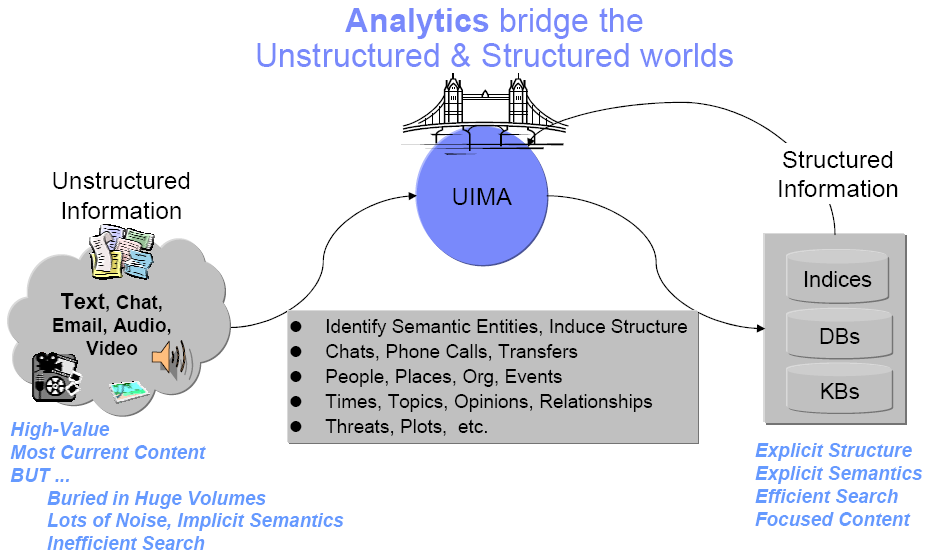
\includegraphics[width=1\textwidth]{fig/uima.png}
    \caption[Short caption]{UIMA: Order unstructured data, from UIMA website \cite{uima:Online}}
    \label{fig:uima}
\end{figure}
\

The real power of UIMA is its Analysis Engines (AE) which basically analyse a document and record descriptive attributes. Those descriptive attributes will form the document's metadata that will be used for further analysis (such as Text Classification in our case).

GIVE EXAMPLES OF AE HERE AND DKPRO PROC PIPILINE AND CAS ?

Thus, the DKPRo software use UIMA's AE in order to collect structured information about textual data. 
\subsection{DKPro Core}
Many NLP tools are already freely available in the NLP research community. DKPro Core \cite{TUD-CS-2014-0864} provides UIMA components wrapping these tools (and some original tools) so they can be used interchangeably in UIMA processing pipelines. The provided components wrap a constantly growing set of stand-of-the-art NLP tools and also include several original components covering a wide range of tasks including: tokenization/segmentation, compound splitting, stemming, part-of-speech tagging, lemmatization, constituency parsing, dependency parsing, named entity recognition, coreference resolution, language identification, spelling correction, grammar checking, and support for reading and writing various file and corpus formats. 
\
\begin{figure}[H]
    \centering
    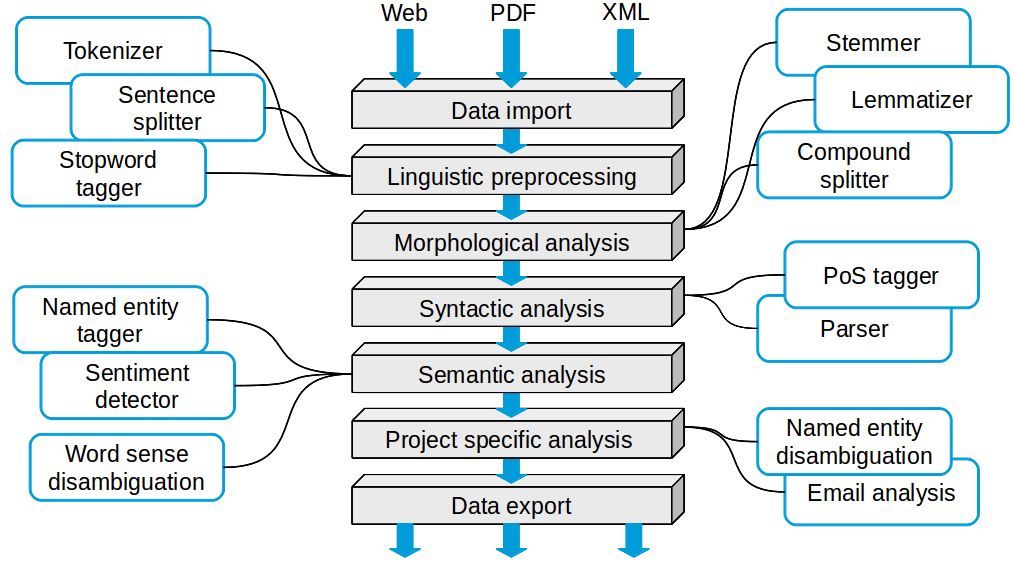
\includegraphics[width=1\textwidth]{fig/dkpro-pipeline.png}
    \caption[Short caption]{DKPro Core Pipeline}
    \label{fig:dkpro-pipeline}
\end{figure}
\
Core has several annotators either developed in-house or wrapped\footnote{A wrapper function is a subroutine in a software library or a computer program whose main purpose is to call a second subroutine or a system call with little or no additional computation. Source: Wikipedia} from the state-of-the-art NLP libraries. Here is a non exhaustive list:
\begin{itemize}
  \item \textbf{Stanford NLP} - segmentation, la lemmatisation, part of speech...
  \item \textbf{OpenNLP} - machine learning based toolkit for the processing of natural language text: tokenization, sentence segmentation, part-of-speech tagging, named entity extraction, chunking, parsing, and coreference resolution. 
  \item \textbf{CleanNLP} - robust NLP components implemented in Java for part-of-speech tagging, dependency parsing, semantic role labelling... 
\end{itemize}

\subsection{DKPro Text Classification}
The aim of DKPro TC (commonly called TC) is to allow the user to apply machine learning algorithms easily on the extracted annotations. This framework was built in order to execute the following tasks:
\begin{itemize}
  \item \Gls{supervised learning} Classification. The user should provide annotated textual data.
  \item Can work atomically on text (word, sentence, paragraph) or on pairs of documents.
  \item Can perform single-label classification, multi-label classification and regression. DEFS
\end{itemize}

Concerning the algorithms used, TC relies on Weka\footnote{http://www.cs.waikato.ac.nz/ml/weka/} (\textit{Waikato Environment for Knowledge Analysis}). Developed by the Waikato University in New Zealand, Weka is an open-source Data Mining software written in Java, which makes available to its users not only Machine Learning algorithms but also processing features (attribute selections and transformations) and a user interface with visualization tools. Regularly updated, Weka is one of the main state-of-the-art data mining software used in research. 
\

Weka is integrated to TC thank to one major component: the \textbf{feature}. In the code, the feature is usually a class that computes a certain value (ex: length of a post, number of adjectives in a text, ect...) using the annotation provided by the DKPro pipeline. Features can be implemented by polymorphism from the mother-class \textit{FeatureExtractorResource$\_$ImplBase}. The results are then saved in an \textit{ARFF} \footnote{An ARFF (Attribute-Relation File Format) file is an ASCII text file that describes a list of instances sharing a set of attributes.} file, which corresponds to Weka's format files.  
\
\begin{figure}[H]
    \centering
    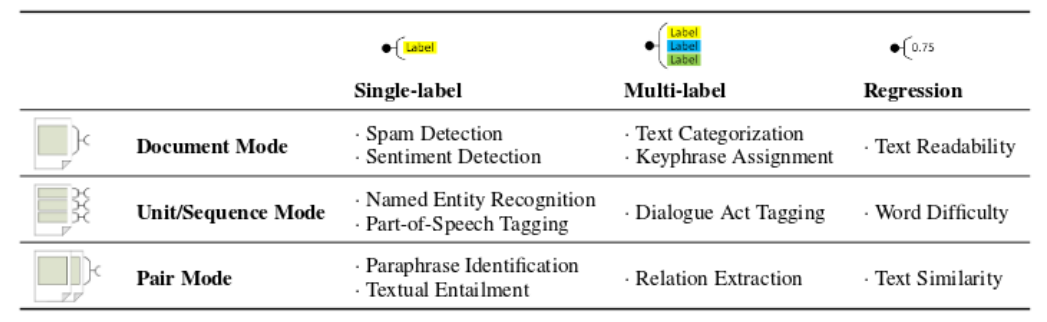
\includegraphics[width=1\textwidth]{fig/TC-modes.png}
    \caption[Short caption]{The different usages of DKPro TC}
    \label{fig:dkpro-tc-usages}
\end{figure}
\

In a nutshell, TC adds 4 more steps to DKPro Core:
  \begin{itemize}
  \item A step where the data are labelled, since we're doing supervised learning. In practice, the label information is extracted my a function of the reader ??WHERE do we define reader ?
  \item Extraction of the features from the annotations.
  \item Data Processing and Cross Validation ??DEF 
  \item Report of the results (Accuracy, Macro F-Measure, ect...)
\end{itemize}  

















